
%(BEGIN_QUESTION)
% Copyright 2006, Tony R. Kuphaldt, released under the Creative Commons Attribution License (v 1.0)
% This means you may do almost anything with this work of mine, so long as you give me proper credit

Kretsen under er for en forenklet 2-leder 4-20mA temperatur transmitter. 

$$\includegraphics[width=15.5cm]{i00397x01.eps}$$

\vskip 10pt

Resten av kretsen ser slik ut:

$$\includegraphics[width=15.5cm]{i00397x02.eps}$$

Regn ut strømmen ut fra emitter på transistoren inne i transmitteren, gitt følgende betingelser:

\begin{itemize}
\item{} Måleomtåde = 50 to 250 degrees C
\item{} Temperatur for termoelement = 100 degrees C
\item{} Forsyningsspenning = 24.0 volts
\item{} Sløyferesistans = 250 ohms
\item{} Spenningsregulatorens inngangstrøm = 3.7 mA (konstant)
\end{itemize}

Tegn også inn strømretning for alle strømmer inne i transmitteren. 

\underbar{file i00397}
%(END_QUESTION)





%(BEGIN_ANSWER)

$I_E$ = 4.3 mA

$$\includegraphics[width=15.5cm]{i00397x03.eps}$$

\vskip 10pt

Follow-up question: how would the transmitter circuit respond to an increase in temperature sensed by the thermocouple?  How about a decrease in loop power supply voltage (24 volts $\to$ 20 volts)?

\vskip 10pt

Challenge question: it is important for instrument accuracy that we make $R_{bias}$ and $R_{feedback}$ resistors rather large in value.  Explain why.

%(END_ANSWER)





%(BEGIN_NOTES)

Answer to challenge question: note how $R_{bias}$ and $R_{feedback}$ constitute a current path {\it around} the shunt resistor $R_{sense}$, allowing loop current that is unmeasured and therefore uncontrolled.

%INDEX% Basics, 2-wire loop-powered transmitter: electronic circuit analysis

%(END_NOTES)


